%%%%%%%%%%%%%%%%%%%%%%%%%%%%%%%%%%%%%%%%%%%%%%%%%%%%%%%%%%%
%%%%%%%%%%%%%%%%%%%%%%%%%%%%%%%%%%%%%%%%%%%%%%%%%%%%%%%%%%%
%%%%%%%%%%%%%%%%%%%%%%%%%%%%%%%%%%%%%%%%%%%%%%%%%%%%%%%%%%%

%% PREAMBLE! :-)


\documentclass[a4paper, 10pt]{article}

%%% packages - input should be path where your packages.tex file is saved.
%% packages

\usepackage{setspace}

%%%%%%%%%%%%%%%%%%%%%%%%%%%%%%%%%%%%%
\usepackage{sectsty}
\sectionfont{\sffamily\Large}
\subsectionfont{\sffamily}
%%%%%%%%%%%%%%%%%%%%%%%%%%%%%%%%%%%%%
\usepackage[titles]{tocloft}
%%%%%%%%%%%%%%%%%%%%%%%%%%%%%%%%%%%%%

%%% This is a package to use UTF8 CSV files as input and directly convert them to latex tables.
\usepackage{csvsimple}
%https://texblog.org/2012/05/30/generate-latex-tables-from-csv-files-excel/

%%%%%%%%%%%%%%%%%%%%%%%%%%%%%%%%%%%%%
%%%%%%%%%%%%%%%%%%%%%%%%%%%%%%%%%%%%%
%%%%%%%%%%%%%%%%%%%%%%%%%%%%%%%%%%%%%

\usepackage[version=4]{mhchem}
% package for using chemical equations and fonts 
% https://mirror.kumi.systems/ctan/macros/latex/contrib/mhchem/mhchem.pdf

%%%%%%%%%%%%%%%%%%%%%%%%%%%%%%%%%%%%%
%%%%%%%%%%%%%%%%%%%%%%%%%%%%%%%%%%%%%
%%%%%%%%%%%%%%%%%%%%%%%%%%%%%%%%%%%%%

\usepackage{xparse}
% high level user interface package, use with caution
% https://mirror.easyname.at/ctan/macros/latex/contrib/l3packages/xparse.pdf

%%%%%%%%%%%%%%%%%%%%%%%%%%%%%%%%%%%%%
%%%%%%%%%%%%%%%%%%%%%%%%%%%%%%%%%%%%%
%%%%%%%%%%%%%%%%%%%%%%%%%%%%%%%%%%%%%

\usepackage{makeidx}
\usepackage{pdfpages}
\usepackage{lastpage}

%%%%%%%%%%%%%%%%%%%%%%%%%%%%%%%%%%%%%
%%%%%%%%%%%%%%%%%%%%%%%%%%%%%%%%%%%%%
%%%%%%%%%%%%%%%%%%%%%%%%%%%%%%%%%%%%%

%%% Package to control inclusion and exclusion of specific entry in the table of contents.
%%% https://mirror.foobar.to/CTAN/macros/latex/contrib/tocbibind/tocbibind.pdf
\usepackage[nottoc,notlot,notlof]{tocbibind}

%%%%%%%%%%%%%%%%%%%%%%%%%%%%%%%%%%%%%
%%%%%%%%%%%%%%%%%%%%%%%%%%%%%%%%%%%%%
%%%%%%%%%%%%%%%%%%%%%%%%%%%%%%%%%%%%%

\usepackage{bigstrut}
% needed for crazy table commands, its cool trust me!
% https://anorien.csc.warwick.ac.uk/mirrors/CTAN/macros/latex/contrib/multirow/multirow.pdf

%%%%%%%%%%%%%%%%%%%%%%%%%%%%%%%%%%%%%
%%%%%%%%%%%%%%%%%%%%%%%%%%%%%%%%%%%%%
%%%%%%%%%%%%%%%%%%%%%%%%%%%%%%%%%%%%%

\usepackage{graphicx} 								
% Required for the inclusion of images
% https://de.overleaf.com/learn/latex/Inserting_Images

%%%%%%%%%%%%%%%%%%%%%%%%%%%%%%%%%%%%%
%%%%%%%%%%%%%%%%%%%%%%%%%%%%%%%%%%%%%
%%%%%%%%%%%%%%%%%%%%%%%%%%%%%%%%%%%%%

\usepackage{amsmath} 								
% Required for some math elements 
% https://www.namsu.de/Extra/pakete/amsmath/Amsmath.html

%%%%%%%%%%%%%%%%%%%%%%%%%%%%%%%%%%%%%
%%%%%%%%%%%%%%%%%%%%%%%%%%%%%%%%%%%%%
%%%%%%%%%%%%%%%%%%%%%%%%%%%%%%%%%%%%%

\usepackage{amssymb}
% required for some more crazy math elements, checks mal ab!
% http://milde.users.sourceforge.net/LUCR/Math/mathpackages/amssymb-symbols.pdf

%%%%%%%%%%%%%%%%%%%%%%%%%%%%%%%%%%%%%
%%%%%%%%%%%%%%%%%%%%%%%%%%%%%%%%%%%%%
%%%%%%%%%%%%%%%%%%%%%%%%%%%%%%%%%%%%%

%\usepackage{kbordermatrix} 	
% some special matrix-commands						
% http://www.hss.caltech.edu/~kcb/TeX/kbordermatrix.sty
%%%%%%%%%%%%%%%%%%%%%%%%%%%%%%%%%%%%%
%%%%%%%%%%%%%%%%%%%%%%%%%%%%%%%%%%%%%
%%%%%%%%%%%%%%%%%%%%%%%%%%%%%%%%%%%%%

\usepackage{multicol}								
% multicolumn-commands stuffs
% https://de.overleaf.com/learn/latex/Multiple_columns

%%%%%%%%%%%%%%%%%%%%%%%%%%%%%%%%%%%%%
%%%%%%%%%%%%%%%%%%%%%%%%%%%%%%%%%%%%%
%%%%%%%%%%%%%%%%%%%%%%%%%%%%%%%%%%%%%

\usepackage{color}
\definecolor{dkgreen}{rgb}{0,0.6,0}
\definecolor{gray}{rgb}{0.5,0.5,0.5}
\definecolor{mauve}{rgb}{0.58,0,0.82}
\definecolor{darkblue}{rgb}{0.0,0.0,0.6}
\definecolor{cyan}{rgb}{0.0,0.6,0.6}

%%%%%%%%%%%%%%%%%%%%%%%%%%%%%%%%%%%%%
%%%%%%%%%%%%%%%%%%%%%%%%%%%%%%%%%%%%%
%%%%%%%%%%%%%%%%%%%%%%%%%%%%%%%%%%%%%

% package to more precisely wrap your document around ur figure!
% https://de.overleaf.com/learn/latex/wrapping_text_around_figures
\usepackage{wrapfig}								

%%%%%%%%%%%%%%%%%%%%%%%%%%%%%%%%%%%%%
%%%%%%%%%%%%%%%%%%%%%%%%%%%%%%%%%%%%%
%%%%%%%%%%%%%%%%%%%%%%%%%%%%%%%%%%%%%

% the package for bold math symbol commands!
% https://anorien.csc.warwick.ac.uk/mirrors/CTAN/macros/latex/required/tools/bm.pdf
\usepackage{bm}

%%%%%%%%%%%%%%%%%%%%%%%%%%%%%%%%%%%%%
%%%%%%%%%%%%%%%%%%%%%%%%%%%%%%%%%%%%%
%%%%%%%%%%%%%%%%%%%%%%%%%%%%%%%%%%%%%

% subcaption package dependant on caption package (self-explanatory)
% https://www.namsu.de/Extra/pakete/Subcaption.html

\usepackage{caption}
\usepackage{subcaption}

%%%%%%%%%%%%%%%%%%%%%%%%%%%%%%%%%%%%%
%%%%%%%%%%%%%%%%%%%%%%%%%%%%%%%%%%%%%
%%%%%%%%%%%%%%%%%%%%%%%%%%%%%%%%%%%%%

%package for appendix control
% https://mirror.easyname.at/ctan/macros/latex/contrib/appendix/appendix.pdf
\usepackage[toc,page]{appendix}

%%%%%%%%%%%%%%%%%%%%%%%%%%%%%%%%%%%%%
%%%%%%%%%%%%%%%%%%%%%%%%%%%%%%%%%%%%%
%%%%%%%%%%%%%%%%%%%%%%%%%%%%%%%%%%%%%

% This is the listings package to make code appear like actual code!
% https://mirror.foobar.to/CTAN/macros/latex/contrib/listings/listings.pdf
\usepackage{listings}{
 \lstset{frame=tb,
  basicstyle=\fontsize{8}{10}\selectfont\sffamily,
  frame=single,	 
  language=Python,
  breaklines=true,
  showstringspaces=false,
  columns=flexible,
  numbers=left,
  commentstyle=\color{dkgreen},
  stringstyle=\color{mauve},
  tabsize=2
}

%%%%%%%%%%%%%%%%%%%%%%%%%%%%%%%%%%%%%
%%%%%%%%%%%%%%%%%%%%%%%%%%%%%%%%%%%%%
%%%%%%%%%%%%%%%%%%%%%%%%%%%%%%%%%%%%%

% this package for more elaborate appendix commands!
% http://mirror.ox.ac.uk/sites/ctan.org/macros/latex/contrib/appendix/appendix.pdf
\usepackage[toc,page]{appendix}
%\renewcommand{\appendixpagename}{\appendixname}
%\renewcommand{\appendixtocname}{\appendixname}

%%%%%%%%%%%%%%%%%%%%%%%%%%%%%%%%%%%%%
%%%%%%%%%%%%%%%%%%%%%%%%%%%%%%%%%%%%%
%%%%%%%%%%%%%%%%%%%%%%%%%%%%%%%%%%%%%

% this is the hyperlink references package! To make stuff in your text clickable and send you to the right page, URL's, E-mails etc..
% http://mirror.ox.ac.uk/sites/ctan.org/macros/latex/contrib/hyperref/doc/manual.pdf
\usepackage[
    bookmarks,
    bookmarksopen=true,
    colorlinks=true,			% diese Farbdefinitionen zeichnen Links im PDF farblich aus
    linkcolor=black, 			% einfache interne Verknüpfungen
    anchorcolor=black,			% Ankertext
    citecolor=black, 			% Verweise auf Literaturverzeichniseinträge im Text
    filecolor=magenta, 			% Verknüpfungen, die lokale Dateien öffnen
    menucolor=red, 				% Acrobat-Menüpunkte
    urlcolor=blue,				% URL color of course :P
    plainpages=false,		 	% zur korrekten Erstellung der Bookmarks
    pdfpagelabels, 				% zur korrekten Erstellung der Bookmarks
    hypertexnames=true, 		% zur korrekten Erstellung der Bookmarks
    %linktocpage 				% Seitenzahlen anstatt Text im Inhaltsverzeichnis verlinken
]{hyperref}

\usepackage{tcolorbox}
%Fancy boxes around text!
%%%%%%%%%%%%%%%%%%%%%%%%%%%%%%%%%%%%%

\usepackage{amsthm}
\usepackage{algorithm}
\usepackage{algpseudocode}
\usepackage{tikz}

%%% Settings!
%% settings
%change relevant macros like title, names etc.

\newcommand{\firstauthorfirstname}{Camilo }
\newcommand{\firstauthorlastname}{Tello Fachin }

\newcommand{\secondauthorfirstname}{Second }
\newcommand{\secondauthorlastname}{Author }

\newcommand{\doctitle}{Exercise 1}

\makeindex
%%%%%%%%%%%%%%%%%%%%%%%%%%%%%%%%%%%%%%%%%%%%%%%%%%%%%%%%%%%%%%%%%%%%%%%%%
%%%%%%%%%%%%%%%%%%%%%%%%%%%%%%%%%%%%%%%%%%%%%%%%%%%%%%%%%%%%%%%%%%%%%%%%%
%%%%%%%%%%%%%%%%%%%%%%%%%%%%%%%%%%%%%%%%%%%%%%%%%%%%%%%%%%%%%%%%%%%%%%%%%

% set the margins of the document, single first input generates evenly spaced margins of that value
\usepackage[margin=2.5cm]{geometry}

%%%%%%%%%%%%%%%%%%%%%%%%%%%%%%%%%%%%%%%%%%%%%%%%%%%%%%%%%%%%%%%%%%%%%%%%%
%%%%%%%%%%%%%%%%%%%%%%%%%%%%%%%%%%%%%%%%%%%%%%%%%%%%%%%%%%%%%%%%%%%%%%%%%
%%%%%%%%%%%%%%%%%%%%%%%%%%%%%%%%%%%%%%%%%%%%%%%%%%%%%%%%%%%%%%%%%%%%%%%%%

\usepackage[utf8]{inputenc}
% u need this one to compile ä ö ü while babel-package is disabled!(english document)!!
% https://www.namsu.de/Extra/pakete/Inputenc.html

%\usepackage[ngerman]{babel}
% uncomment this package to have all the generated text lik TOC and TOC-APP in german
% IF U UNCOMMENT THIS, PUT THE UTF8 INPUTENC PACKAGE IN COMMENT
% https://www.namsu.de/Extra/pakete/German.html

%%%%%%%%%%%%%%%%%%%%%%%%%%%%%%%%%%%%%%%%%%%%%%%%%%%%%%%%%%%%%%%%%%%%%%%%%
%%%%%%%%%%%%%%%%%%%%%%%%%%%%%%%%%%%%%%%%%%%%%%%%%%%%%%%%%%%%%%%%%%%%%%%%%
%%%%%%%%%%%%%%%%%%%%%%%%%%%%%%%%%%%%%%%%%%%%%%%%%%%%%%%%%%%%%%%%%%%%%%%%%


% header and footer settings
% to look up stuff on it go visit this one:
% https://en.wikibooks.org/wiki/LaTeX/Customizing_Page_Headers_and_Footers

\usepackage{fancyhdr}
\setlength{\headheight}{22.25pt}

\renewcommand{\headrulewidth}{0.5pt}
\renewcommand{\footrulewidth}{0.5pt}

\pagestyle{fancy}


% header inputs
\lhead[even output]{HPC}
\chead[even output]{Exercise 1}
\rhead[even output]{
\includegraphics[width=2.5cm]{figures/uni_header}}


%footer inputs
\lfoot[even output]{CSE - WS22}
\cfoot[even output]{Page  \thepage}
\rfoot[even output]{\today}

%%%%%%%%%%%%%%%%%%%%%%%%%%%%%%%%%%%%%%%%%%%%%%%%%%%%%%%%%%%%%%%%%%%%%%%%%
%%%%%%%%%%%%%%%%%%%%%%%%%%%%%%%%%%%%%%%%%%%%%%%%%%%%%%%%%%%%%%%%%%%%%%%%%
%%%%%%%%%%%%%%%%%%%%%%%%%%%%%%%%%%%%%%%%%%%%%%%%%%%%%%%%%%%%%%%%%%%%%%%%%


%settings for PDF metadata, available if rightclick on pdf in adobe and chose properties!

\hypersetup{pdfinfo={
Title={\doctitle},
Subject={High Performance Computing},
Author={Camilo Tello Fachin},
Keywords={Concurrent Programs, }{Parallel Programming, }{Technical University Vienna, }{Winter Semester 22, }
{MSc Computational Science and Engineering}
}}

%%%%%%%%%%%%%%%%%%%%%%%%%%%%%%%%%%%%%%%%%%%%%%%%%%%%%%%%%%%%%%%%%%%%%%%%%
%%%%%%%%%%%%%%%%%%%%%%%%%%%%%%%%%%%%%%%%%%%%%%%%%%%%%%%%%%%%%%%%%%%%%%%%%
%%%%%%%%%%%%%%%%%%%%%%%%%%%%%%%%%%%%%%%%%%%%%%%%%%%%%%%%%%%%%%%%%%%%%%%%%

%% This is the bibliography package,
\usepackage[
backend=bibtex,
style=ieee,
sorting=ynt,
backref=false,
hyperref=true
]{biblatex}

%%%%%%%%%%%%%%%%%%%%%%%%%%%%%%%%%%%%%%%%%%%%%%%%%%%%%%%%%%%%%%%%%%%%%%%%%
%%%%%%%%%%%%%%%%%%%%%%%%%%%%%%%%%%%%%%%%%%%%%%%%%%%%%%%%%%%%%%%%%%%%%%%%%
%%%%%%%%%%%%%%%%%%%%%%%%%%%%%%%%%%%%%%%%%%%%%%%%%%%%%%%%%%%%%%%%%%%%%%%%%

%%% This is an important setting which lets u control the spacing between lines! Just comment/uncomment the desired ones!


%\singlespacing

\onehalfspacing

%\doublespacing

%%%%%%%%%%%%%%%%%%%%%%%%%%%%%%%%%%%%%%%%%%%%%%%%%%%%%%%%%%%%%%%%%%%%%%%%%

%%% custom commands

\newcommand{\var}[1]{\texttt{#1}}
\newcommand{\fun}[1]{\texttt{#1}}
\newcommand{\obj}[1]{\texttt{#1}}

\newtheorem*{theorem*}{Theorem}
\newtheorem*{proof*}{Proof}

%%% macros - where u define ur macros and newcommands!
% useful macros!


% insert a blank page which is still counted
\newcommand{\blankpage}{
\newpage
\thispagestyle{empty}
\mbox{}
\newpage
}

%%% the bibliohraphy! the settings to the bibliography are changed in the packages.tex file, where the bibtex package is loaded!
\addbibresource{content/04_bibliography.bib}

\begin{document}


%%%%%%%%%%%%%%%%%%%%%%%%%%%%%%%%%%%%%%%%%%%%%%%%%%%%%%%%%%%
%%%%%%%%%%%%%%%%%%%%%%%%%%%%%%%%%%%%%%%%%%%%%%%%%%%%%%%%%%%%
%%%%%%%%%%%%%%%%%%%%%%%%%%%%%%%%%%%%%%%%%%%%%%%%%%%%%%%%%%%
          

\begin{titlepage}

\newcommand{\HRule}{\rule{\linewidth}{0.5mm}} % Defines a new command for the horizontal lines, change thickness here

\center % Center everything on the page
 
%----------------------------------------------------------------------------------------
%	HEADING SECTIONS
%----------------------------------------------------------------------------------------

\textsc{\LARGE Vienna University of Technology}\\[1.5cm] % Name of your university/college
\textsc{\Large 184.725 High Performance Computing}\\[0.5cm] % Major heading such as course name
\textsc{\large TU Wien Informatics}\\[0.5cm] % Minor heading such as course title

%----------------------------------------------------------------------------------------
%	TITLE SECTION
%----------------------------------------------------------------------------------------

\HRule \\[0.5cm]
{ \huge \bfseries \doctitle}\\[1mm] % Title of your document
\HRule \\[0.5cm]
 
%----------------------------------------------------------------------------------------
%	AUTHOR SECTION
%----------------------------------------------------------------------------------------

\begin{minipage}{0.4\textwidth}
\begin{flushleft} \large
\emph{Authors:}\\
Camilo \textsc{Tello Fachin}\\
12127084 \\
Manuela Maria \textsc{Raidl}\\
01427517 \\

\end{flushleft}
\end{minipage}
~
\begin{minipage}{0.4\textwidth}
\begin{flushright} \large
\emph{Supervisor:} \\
Prof. Dr. Jesper Larsson \textsc{Träff} \\ % Supervisor's Name
\end{flushright}
\end{minipage}\\[1.5cm]

% If you don't want a supervisor, uncomment the two lines below and remove the section above
%\Large \emph{Author:}\\
%John \textsc{Smith}\\[3cm] % Your name

%----------------------------------------------------------------------------------------
%	DATE SECTION
%----------------------------------------------------------------------------------------

{\large \today}\\[1.5cm] % Date, change the \today to a set date if you want to be precise

%----------------------------------------------------------------------------------------
%	LOGO SECTION
%----------------------------------------------------------------------------------------
\vfill


\includegraphics[width=0.75\textwidth]{figures/uni_titlepage}\\[5cm] % Include a department/university logo
 
%----------------------------------------------------------------------------------------

\vfill % Fill the rest of the page with whitespace
\pagenumbering{alph}

\end{titlepage} 

%\blankpage

% this is to remove the first paragraph sentence indentation! if you want indentation, set the second input to the desired indendation value.
\setlength{\parindent}{0pt}

% this file is loaded, to include PDF's such as declaration of intent for theses, abstracts and summaries in other languages.
\pagenumbering{roman}

\section*{Abstract}
Here documented the results of exercise 6.



%%% If your TOC is too large for one page, you can distribute it over 2 pages and comment this /blankpage command below! To better control the distribution of the content of the table of content, use the geometry settings and adjust the top and bottom margin for the table of content in the next part of this code.

%\blankpage



%%% Here u define the TOC, a newgeometry command is used to let you design your own TOC margins. just comment out the \newgeometry and the \restoregeometry
%%% command to force the same margins as the rest of the document to the TOC

\pagebreak
\thispagestyle{empty}
\newgeometry{top=2.25cm, bottom=2.25cm}
{\sffamily\tableofcontents}
\thispagestyle{empty}
\restoregeometry
\pagebreak

\pagenumbering{arabic}


%%%%%%%%%%%%%%%%%%%%%%%%%%%%%%%%%%%%%%%%%%%%%%%%%%%%%%%%%%%
%%%%%%%%%%%%%%%%%%%%%%%%%%%%%%%%%%%%%%%%%%%%%%%%%%%%%%%%%%%
%%%%%%%%%%%%%%%%%%%%%%%%%%%%%%%%%%%%%%%%%%%%%%%%%%%%%%%%%%%
%%%%%%%%%%%%%%%%%%%%%%%%%%%%%%%%%%%%%%%%%%%%%%%%%%%%%%%%%%%



%%% This is a first surrogate chapter to intuitively show you how and where to include new chapters!asd
%\section*{To Do's}

- What's still to you do make your supervisor/prof happy?
\pagebreak





%\pagebreak

\section{Exercise 1 - Closed Form Expressions}
\subsection{$\sum_{i=0}^d k^i \quad \mathrm{for } \, k>0$ (Ex1.1)}
\begin{equation}
\begin{aligned}
    \sum_{i=0}^d k^i &= \sum_{i=0}^d k^i \\
    \sum_{i=0}^d k^i - k \sum_{i=0}^d k^i &= \sum_{i=0}^d k^i - k \sum_{i=0}^d k^i \\
    \sum_{i=0}^d k^i - k \sum_{i=0}^d k^i &= \sum_{i=0}^d k^i - \sum_{i=1}^{d+1} k^i \\
    \sum_{i=0}^d k^i \, (1-k) &= 1 - k^{d+1}\\
    \sum_{i=0}^d k^i   &=  \frac{k^{d+1} - 1}{k-1}
    \label{closedForm_Ex1.1}
\end{aligned}
\end{equation}

\subsection{$\sum_{i=1}^d ik^i \quad \mathrm{for } \, k>0$ (Ex1.4)}
\begin{equation}
\begin{aligned}
    \sum_{i=1}^d ik^i &= \sum_{i=0}^d ik^i = 
    \sum_{i=0}^d k \frac{\mathrm{d}}{\mathrm{d}k}k^i =
    k \frac{\mathrm{d}}{\mathrm{d}k} \overbrace{\sum_{i=0}^d k^i}^{\text{use (\ref{closedForm_Ex1.1})}} \\
    \sum_{i=1}^d ik^i &= k \frac{\mathrm{d}}{\mathrm{d}k} \frac{1 - k^{d+1}}{1-k} = 
    \frac{d  k^{d+2} - (d+1)k^{d+1} + k}{(1-k)^2}
    \label{closedForm_Ex1.4}
\end{aligned}
\end{equation}

\subsection{$\sum_{i=1}^d i2^{d-i}$ (Ex1.3)}
\begin{equation}
    \begin{aligned}
        \sum_{i=1}^d i2^{d-i} &, \quad \text{use k instead of 2} \\
        \sum_{i=1}^d ik^{d-i} &= \sum_{i=0}^d dk^{d-i} - \sum_{i=0}^d (d-i)k^{d-i} \\
        &= d\underbrace{\sum_{j=0}^d k^{j}}_{\text{use } (\ref{closedForm_Ex1.1})} - 
        \underbrace{\sum_{j=0}^d jk^{j}}_{\text{use } (\ref{closedForm_Ex1.4})} \quad \text{with } j := d-1 \\
        &= \frac{d(k^{d+1} - 1)}{k-1} - \frac{d  k^{d+2} - (d+1)k^{d+1} + k}{(1-k)^2} \quad \text{set $k$ back to 2} \\
        &= d2^{d+1} - d - d2^{d+2} + d2^{d+1} + 2^{d+1} - 2 \\
        \sum_{i=1}^d i2^{d-i} &= 2^{d+1} -2 - d
        \label{closedForm_Ex1.3}
    \end{aligned}
    \end{equation}

\subsection{$\sum_{i=1}^d i2^i$}

\begin{equation}
    \begin{aligned}
        \sum_{i=1}^d i2^i = d  2^{d+2} - (d+1)2^{d+1} + 2 \quad \text{with use of (\ref{closedForm_Ex1.4})}
    \end{aligned}
\end{equation}

\pagebreak





\section{Exercise 2 - Graph Tree's with Canonical Numbering}
\subsection{$T^d_k$ with $k=3$ and $d=3$}


\subsection{$B^d_k$ with $k=3$ and $d=4$}

\section{Exercise 3 - Planar Graph $H_d$}

\section{Exercise 4 - Gray Code Embedding}
\pagebreak

\section{Exercise 2 - Implement Linear Pipeline for \texttt{MPI\_Bcast} and \texttt{MPI\_Reduce}}

SLIDES ZITIERN, PAPER TRAEFF ZITIERN, REFERENZ ZU NER ANDEREN CHAPTER MACHEN

The goal of exercise 2 is to implement linear pipelined versions of \texttt{MPI\_Bcast()} and \texttt{MPI\_Reduce()} 
based on the algorithms discussed in the lecture (refer to Algorithm 16 and Algorithm 17 of "Algorithms for Collective 
Communication"). \\

Our implementation for the pipelined reduction -- \texttt{MY\_Reduce\_P()} – aligns with the following idea: We 
distinct between a master process (rank $= 0$), interior processes ($0 <$ rand $<$ size $-1$) and an end process 
(rank $=$ size $-1$). As an output of \texttt{MY\_Reduce\_P()}, the master shall possess the entry-wise maximum as 
reduction result. Additionally, we divide the array that needs to be compared into multiple blocks of size 
\texttt{blockSize} (and probably a smaller block in the end). Goal is to communicate between the processes for each 
block separately. \\

The end process (rank $=$ size $-1$) sends blocks – one after the other -- to the interior process with 
rank $=$ size $-2$. The end process does not receive data, as there are no further processes. Interior processes 
first receive a data block from their neighbor with rank $+1$, perform a local reduction and send this data to their 
other neighbor with rank $-1$. This is repeated for all blocks. The master process receives block data from the interior 
node of rank $=1$.\\

Our implementation for the pipelined broadcast -- \texttt{MY\_Bcast\_P()} – is quite similar to the 
\texttt{MY\_Reduce\_P()} implementation. For broadcast the goal is that the data which is I the beginning 
available for the master process shall be communicated to all the other processes. In order to do so, the master 
process sends its data block wise to its neighbor with rank $=1$ (interior process). Interior processes receive block 
data from their predecessor process and immediately communicate this data to their successor process – block by 
block. The last one to receive the data is the end processor. There is no need to send any further data from here.\\

The trivial combination of \texttt{MY\_Reduce\_P()} and \texttt{MY\_Bcast\_P()} can be seen as a pipelined variant 
of \texttt{MPI\_Allreduce()}.\\

\begin{figure}[h]
\begin{center}
    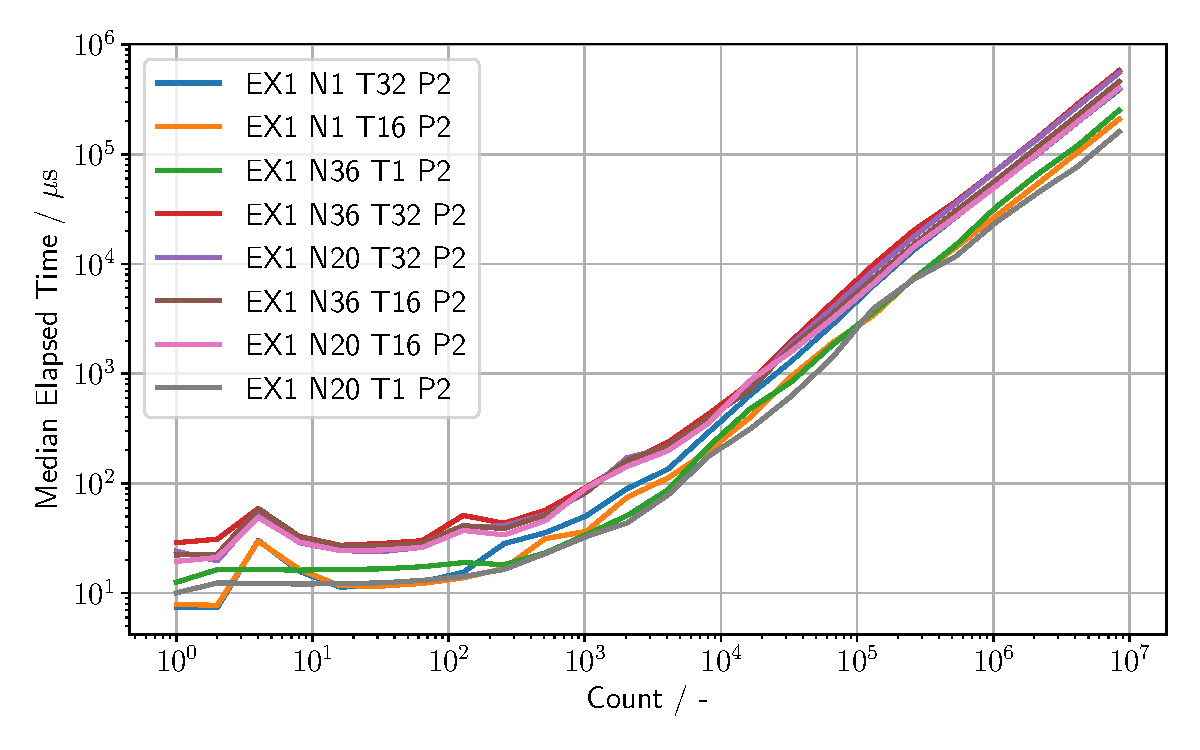
\includegraphics[width=1.0\linewidth]{figures/Ex2_1.pdf}
    \caption{Caption for Ex2 plot 1}
    \label{Ex2_1_p}
\end{center}
\end{figure}

\begin{figure}[h]
\begin{center}
    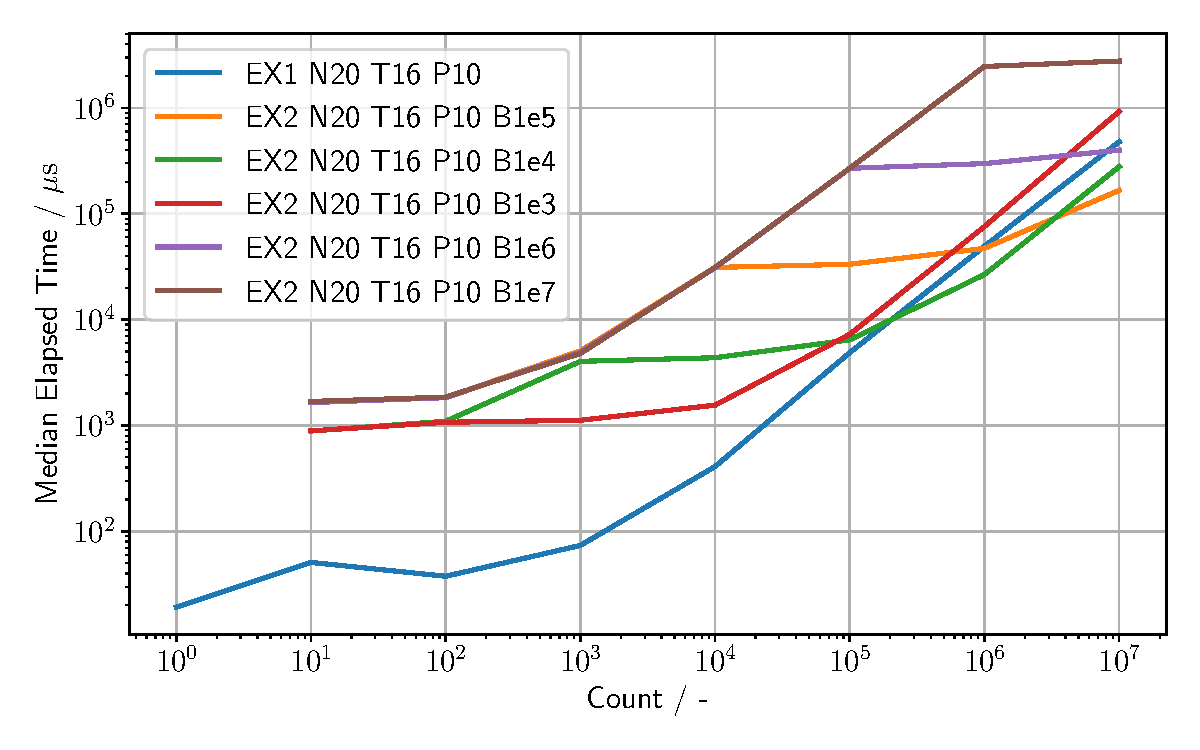
\includegraphics[width=1.0\linewidth]{figures/Ex2_2.pdf}
    \caption{Caption for Ex2 plot 2}
    \label{Ex2_2_p}
\end{center}
\end{figure}

\begin{figure}[h]
\begin{center}
    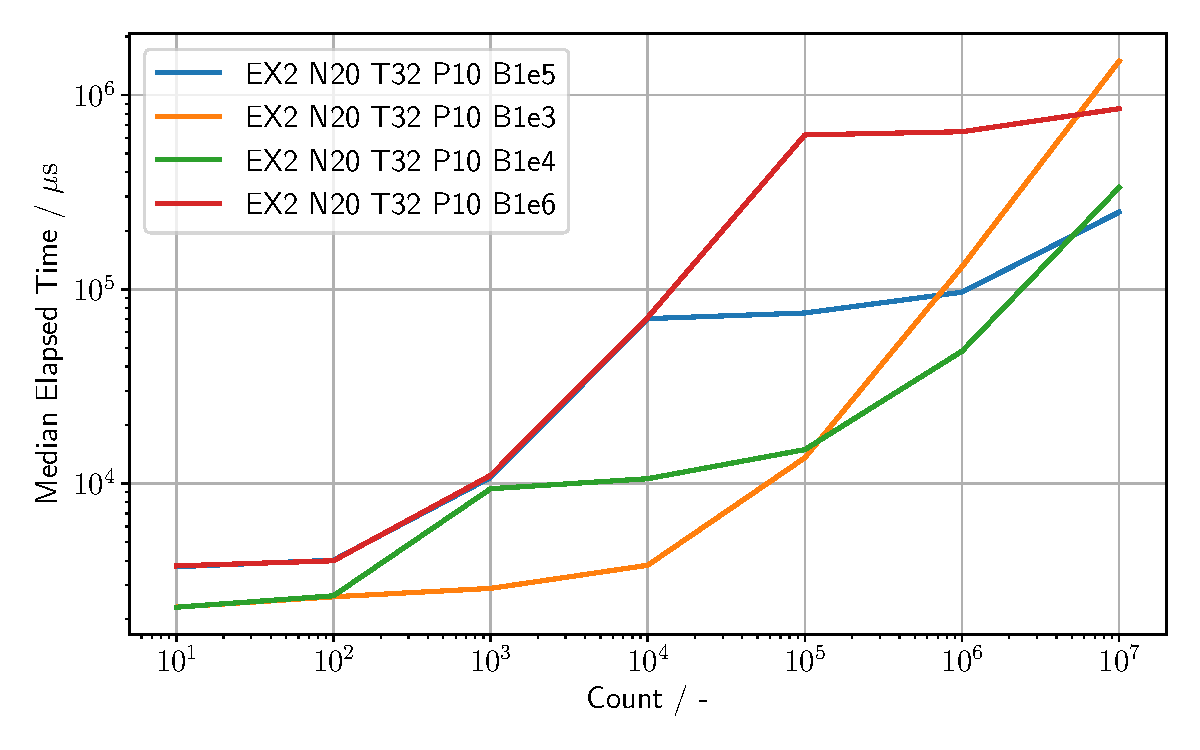
\includegraphics[width=1.0\linewidth]{figures/Ex2_3.pdf}
    \caption{Caption for Ex2 plot 3}
    \label{Ex2_3_p}
\end{center}
\end{figure}

%% 2_4 and 2_5 plots next to each other!

\begin{figure}[h]
\centering
    \begin{minipage}{.5\textwidth}
        \centering
        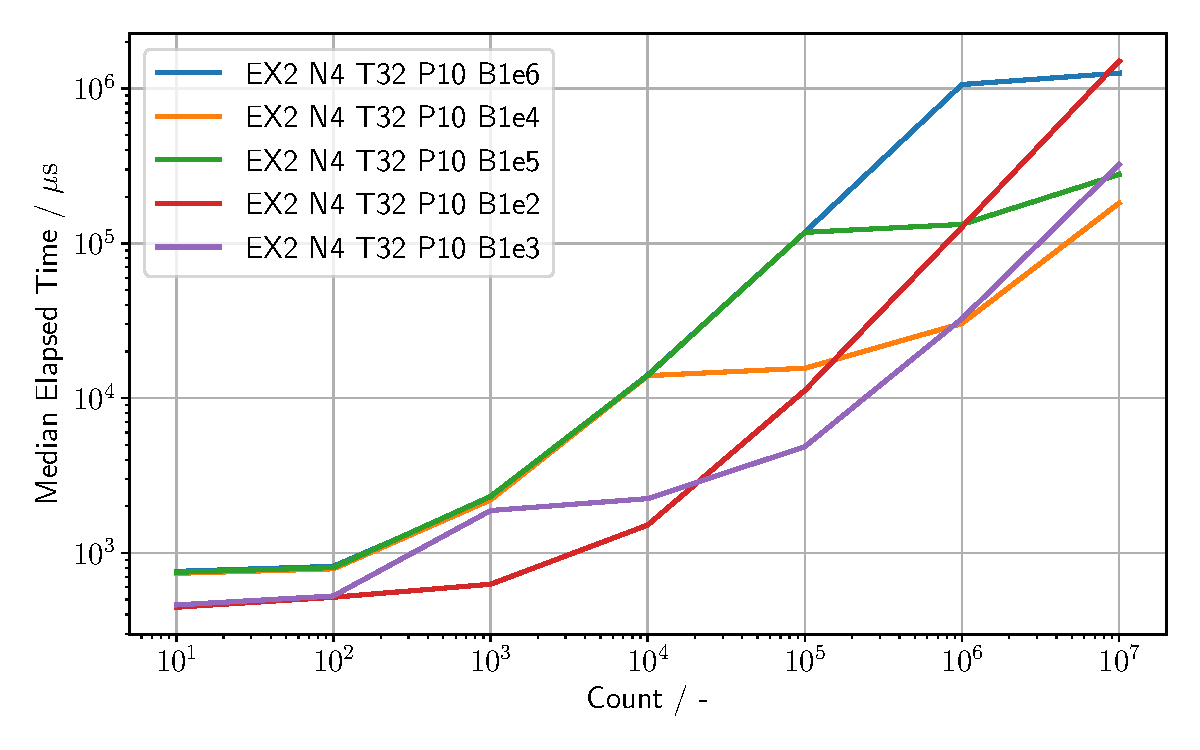
\includegraphics[width=1.0\linewidth]{figures/Ex2_4.pdf}
        \captionof{figure}{Caption for Ex2 plot 4}
        \label{Ex2_4_p}
    \end{minipage}%
    \begin{minipage}{.5\textwidth}
        \centering
        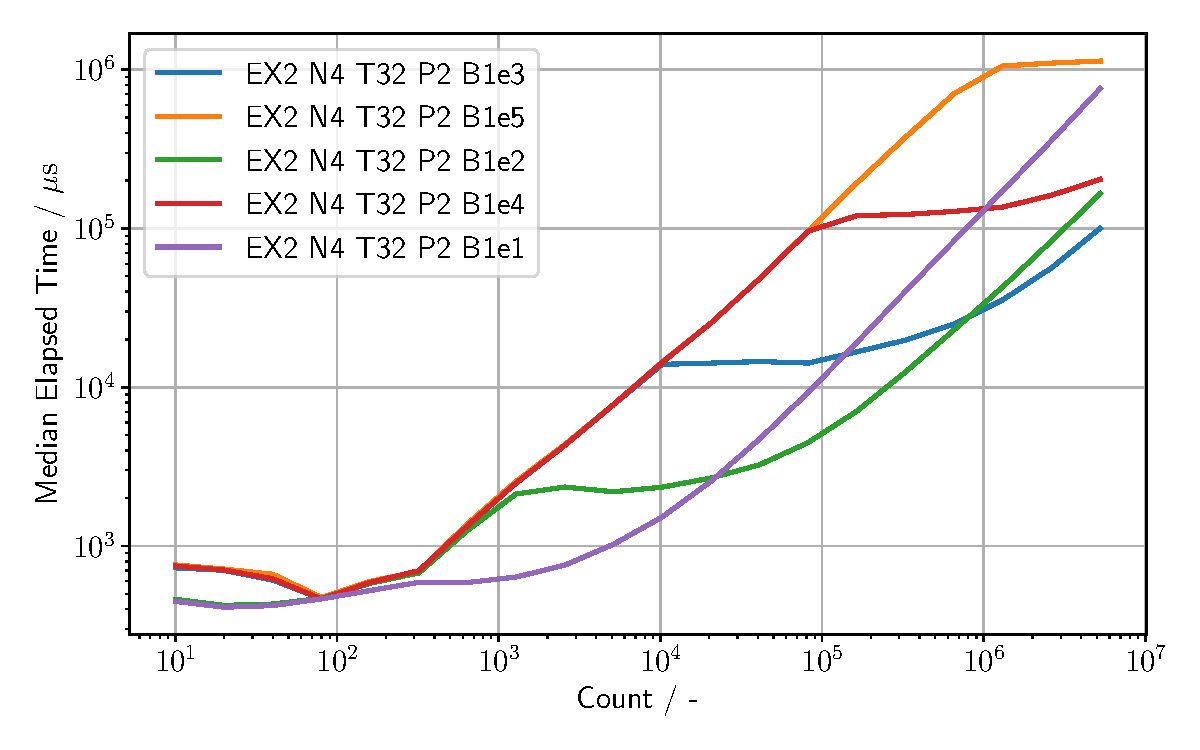
\includegraphics[width=1.0\linewidth]{figures/Ex2_5.pdf}
        \captionof{figure}{Caption for Ex2 plot 5}
        \label{Ex2_5_p}
    \end{minipage}
\end{figure}

% \begin{figure}[h]
%     \begin{center}
%         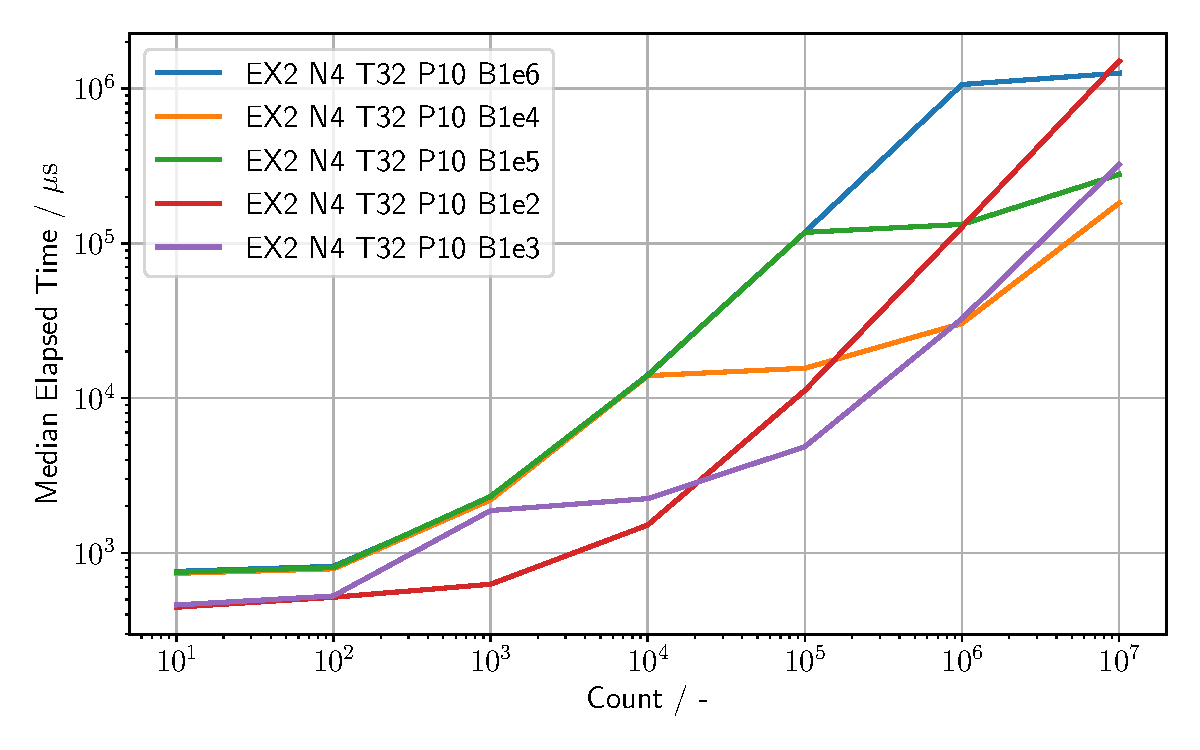
\includegraphics[width=1.0\linewidth]{figures/Ex2_4.pdf}
%         \caption{Caption for Ex2 plot 4}
%         \label{Ex2_4_p}
%     \end{center}
% \end{figure}

% \begin{figure}[h]
%     \begin{center}
%         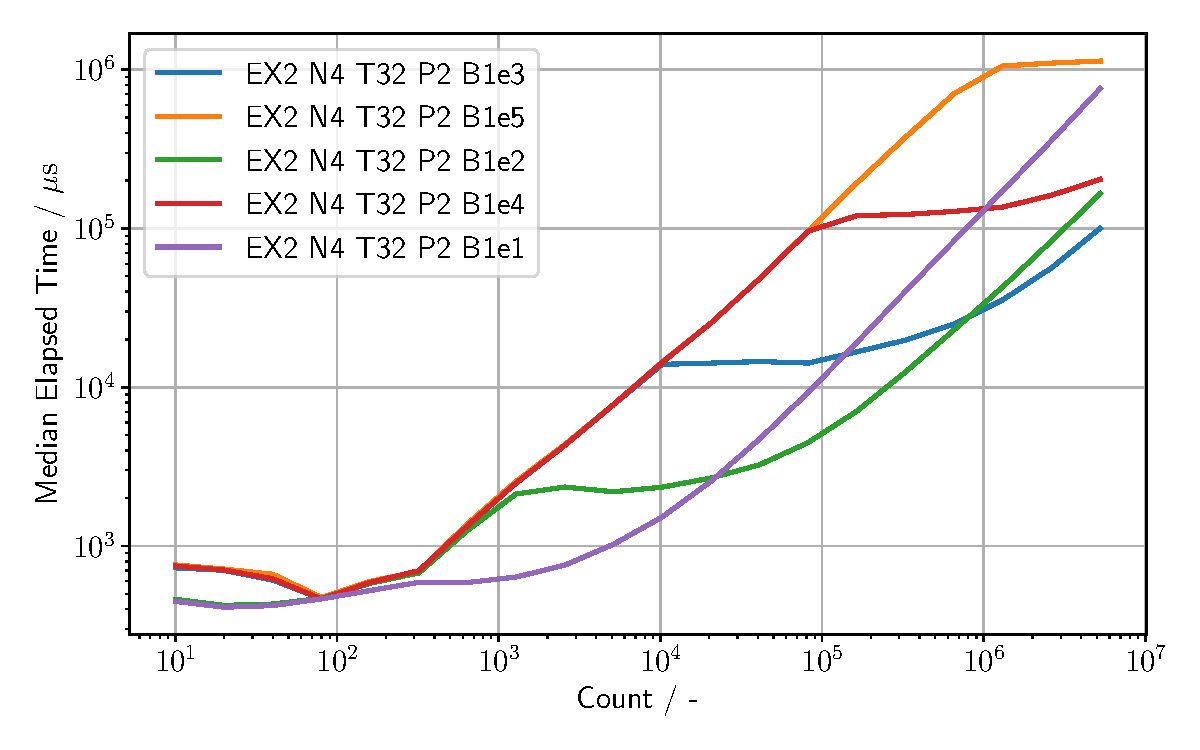
\includegraphics[width=1.0\linewidth]{figures/Ex2_5.pdf}
%         \caption{Caption for Ex2 plot 5}
%         \label{Ex2_5_p}
%     \end{center}
% \end{figure}




\pagebreak

\section{Exercise 3 - Combining \texttt{MPI} Processes}

With the goal of saving slightly on communication rounds by combining a pipelined reduction and a 
pipelined broadcast more tightly to keep the processes “more busy”, we end up with the function implementation 
of \texttt{MY\_Allreduce\_P()}. This implementation is completely based on the pipelined tree 
implementation for exercise 5 (see chapter \ref{chapter_5_reference}). For better understanding, refer to exercise 5 first.\\

Hence, we interpret the “lined up” processes as a tree, where each node except one leaf has exactly 
one child and all nodes except the root have a parent node. With this understanding, we reuse the 
implementation of \texttt{MY\_Allreduce\_T()} from exercise 5 by getting rid of the communication between 
a “right child” and its parent as in our setting for exercise 3 only “left children” exist.\\

We can expect an improvement compared to the trivial combination of \texttt{MY\_Reduce\_P()} and 
\texttt{MY\_Bcast\_P()}, as in \texttt{MY\_Allreduce\_P()} the reduction already gets started as soon 
as the data of the first block received the master process -- the root node. Therefore, 
$\text{number of processes/nodes} - 1 + \text{number of blocks}$ are needed in \texttt{MY\_Allreduce\_P()}, 
whereas \texttt{MY\_Reduce\_P()} and \texttt{MY\_Bcast\_P()} use $\text{number of blocks}$ communication rounds 
each. For a small numbers of processes/nodes, the number of communication rounds can be reduced based 
on the number of blocks and therefore the blocksize. The same structure like in exercise 2 shown
in figure \ref{Ex2_sketch_p} is used here in exercise 3 but now. In exercise 2, the blue arrows (broadcast)
only started sending after ALL blocks where reduced, in exercise 3, the algorithm was designed such that
a block could already be broadcasted once it was reduced, independent of the reduction-state of the other blocks.\\

% For performance estimation let us consider the number of communication rounds between processes in our
% pipelined \texttt{MY\_Allreduce\_P()}. Again let $b$ be the total number of blocks and $n$ the 
% number of processes. Then, there is the need for a total of $b+n-1$ rounds of communication.
% As we assume $n$ to be smaller than the numbers of blocks, we end up with less communication rounds
% copmared to \texttt{MY\_Reduce\_P()} and \texttt{MY\_Bcast\_P()} from exercise 2. 

\pagebreak

For exercise 3 and the following exercises, we have implemented a simple variable blocksize based on the observations
of the timings with different blocksizes in exercise 2.

\null
\null

\begin{lstlisting}[language=C, title=C Code for variable blocksize ]
int get_blockSize(int count){
    if (count < 1e4){
        return 1e2;
    }
    else if (count < 1e6){
        return 1e3;
    }
    else return 1e6;
}
\end{lstlisting}

\null
\null
\null


In the figures below are illustrative results where we compare the performance of exercise 2 and 3. We can observe
that algorithm coded in 3 is not growing performance wise with the time spent coding it. For count $10^3$ the
algorithm of Ex3 outperforms the linearly pipelined one of Ex2.\\


\begin{figure}[h]
    \begin{center}
        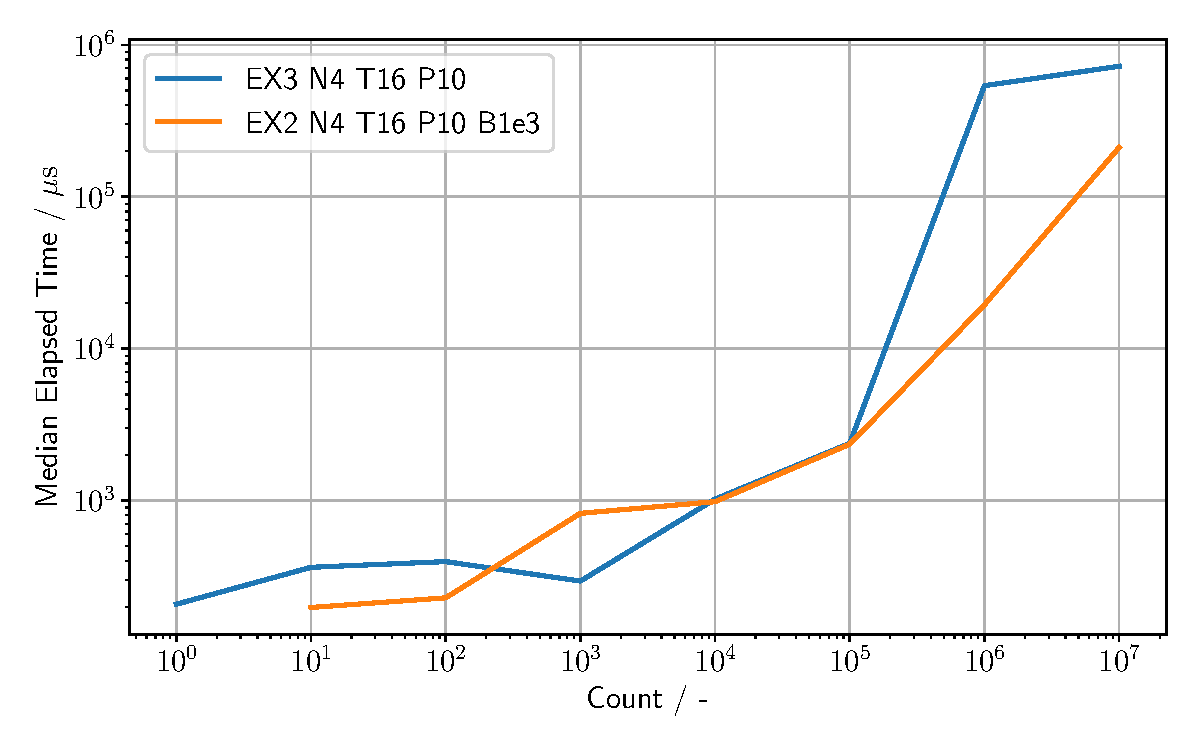
\includegraphics[width=1\linewidth]{figures/Ex3_1.pdf}
        \caption{Median of elapsed time for \fun{MY\_Allreduce\_P()}. 4 nodes, 16 processes per node, powers of 10,
         static blocksize for the EX2 timing and variable blocksize for EX3 timing. 
         20 nodes, 16 processes per node and powers of 10. Performance improvement for count $10^3$.}
        \label{Ex3_1_p}
    \end{center}
\end{figure}

\pagebreak

In figure \ref{Ex3_2_p} we show the configuration of 4 nodes, both powers and all 3 tasks per processes numbers.
It can be seen that the slope decreases again at certain numbers of counts for both powers of 2 and 10, 
this is most likely not due to the improved algorithm, but due to our variable blocksize.

\begin{figure}[h]

    \begin{center}
        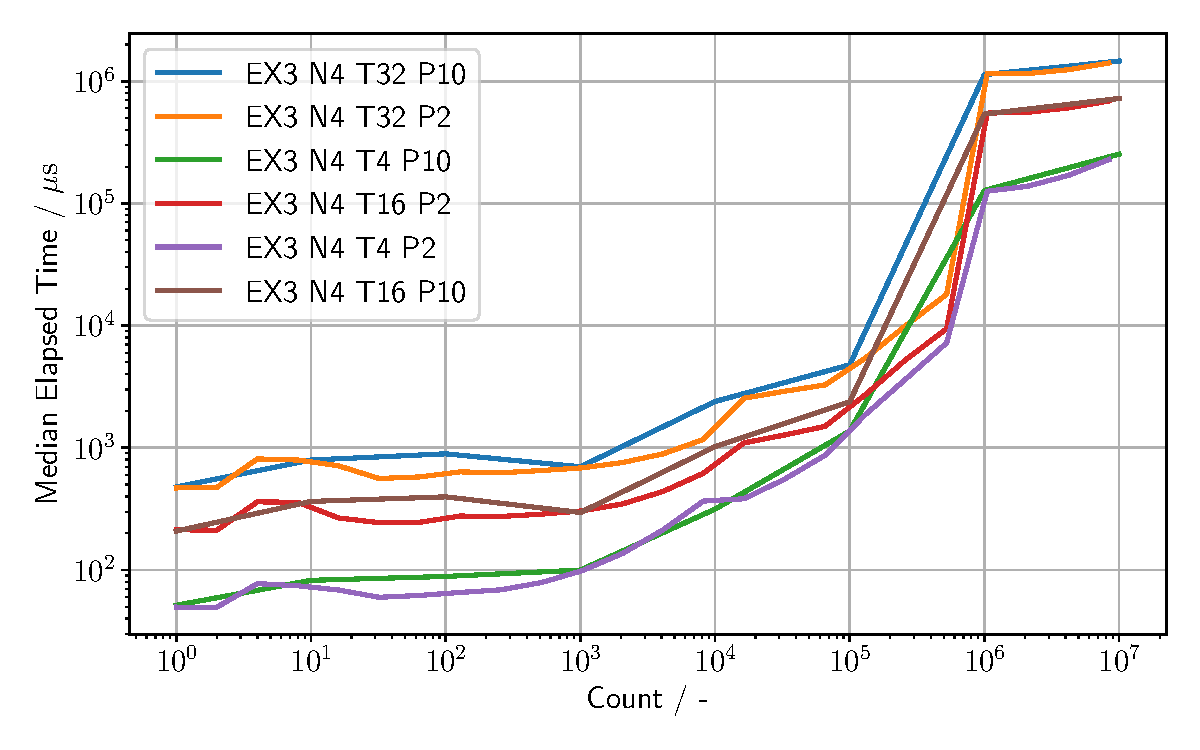
\includegraphics[width=1\linewidth]{figures/Ex3_2.pdf}
        \caption{Median of elapsed time for \fun{MY\_Allreduce\_P()}. 4 nodes, 4 processes per node, 
        powers of 2 and 10, and variable blocksize. Performance improvements visible most likely
        due to variable blocksize.}
        \label{Ex3_2_p}
    \end{center}
\end{figure}

\pagebreak

\section{Exercise 4 - Binary Tree Algorithms for \texttt{MPI\_Bcast} and \texttt{MPI\_Reduce}}
Instead of “lined up” processes we now want to use a binary tree structure and according algorithms 
\texttt{MY\_Reduce\_T()} and \texttt{MY\_Bcast\_T()} for reduction and broadcasting. As we understand 
each process as a node, we will use the wording node from now on. For indexing of the nodes, we use preorder traversal.

We start very similar to the implementations of \texttt{MY\_Reduce\_P()} and \texttt{MY\_Bcast\_P()} 
from exercise 2. For the reduction \texttt{MY\_Reduce\_P()}  the root node (rank $=0$) on level 0 should 
gain the reduced result. Hence, the leaves start by sending the data block by block to their parents. All 
interior nodes receive exactly two data blocks per communication round. One from their left and one from their 
right child. After performing a local reduction, the data is sent to the nodes parent. In the end, the root 
node receives the data from its two children and ends up with the reduction result. For the broadcast 
\texttt{MY\_Bcast\_P()}, the root node sends the data block wise to its two children. A child receives 
the data and immediately forwards this data to its children, in case it is not a leaf.\\

The trivial combination of \texttt{MY\_Reduce\_T()} and \texttt{MY\_Bcast\_T()} can be seen 
as a pipelined variant of \texttt{MPI\_Allreduce()}.\\

\begin{figure}[h]
    \begin{center}
        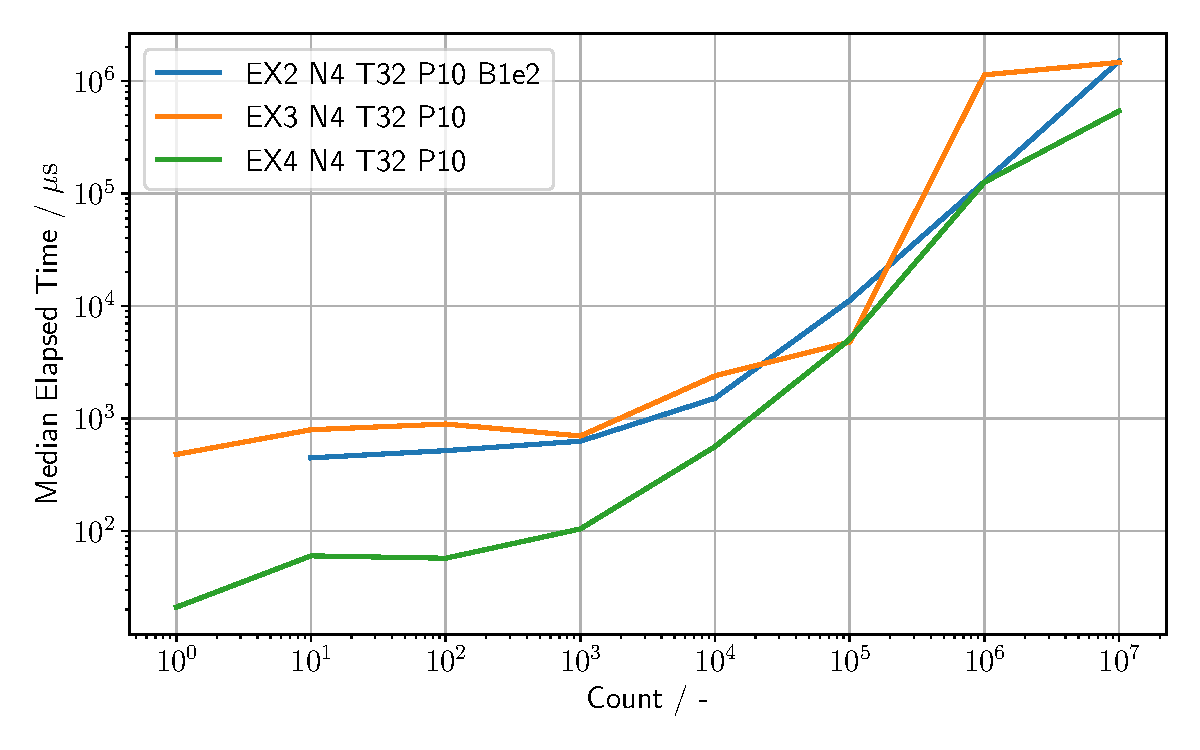
\includegraphics[width=1.0\linewidth]{figures/Ex4_1.pdf}
        \caption{Caption for Ex4 plot 1}
        \label{Ex4_1_p}
    \end{center}
\end{figure}

\begin{figure}[h]
    \begin{center}
        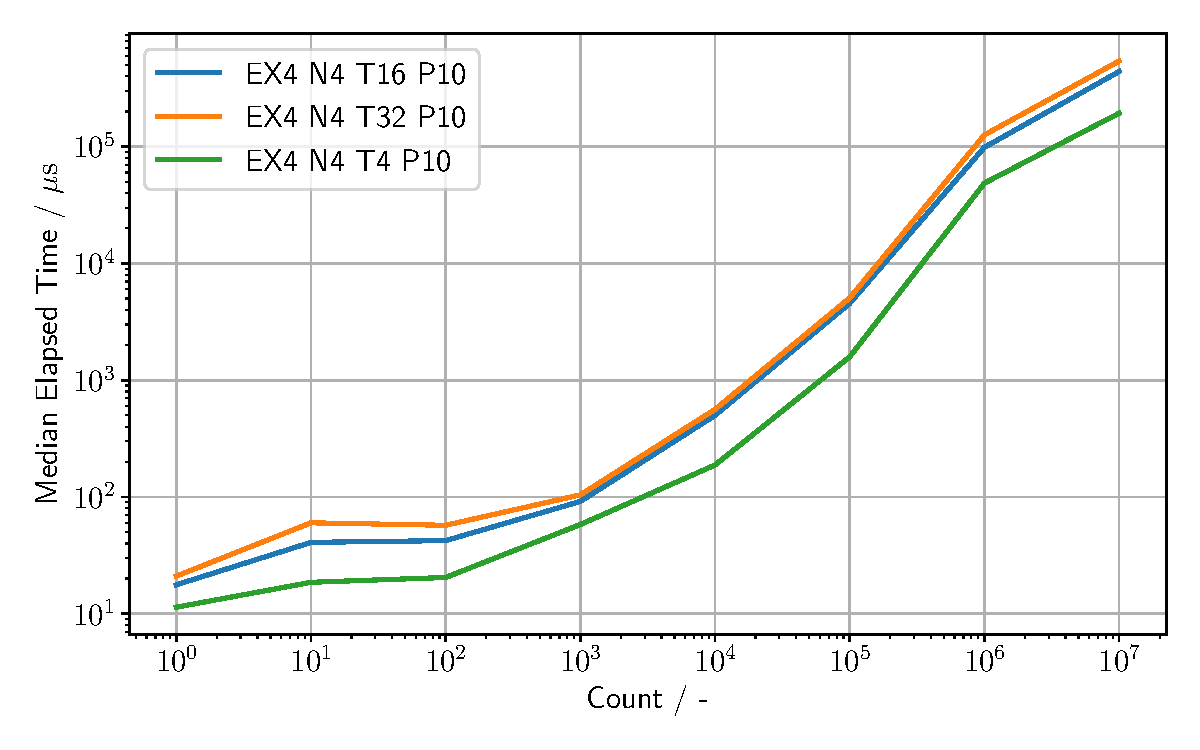
\includegraphics[width=1.0\linewidth]{figures/Ex4_2.pdf}
        \caption{Caption for Ex4 plot 2}
        \label{Ex4_2_p}
    \end{center}
\end{figure}

\begin{figure}[h]
\centering
    \begin{minipage}{.5\textwidth}
        \centering
        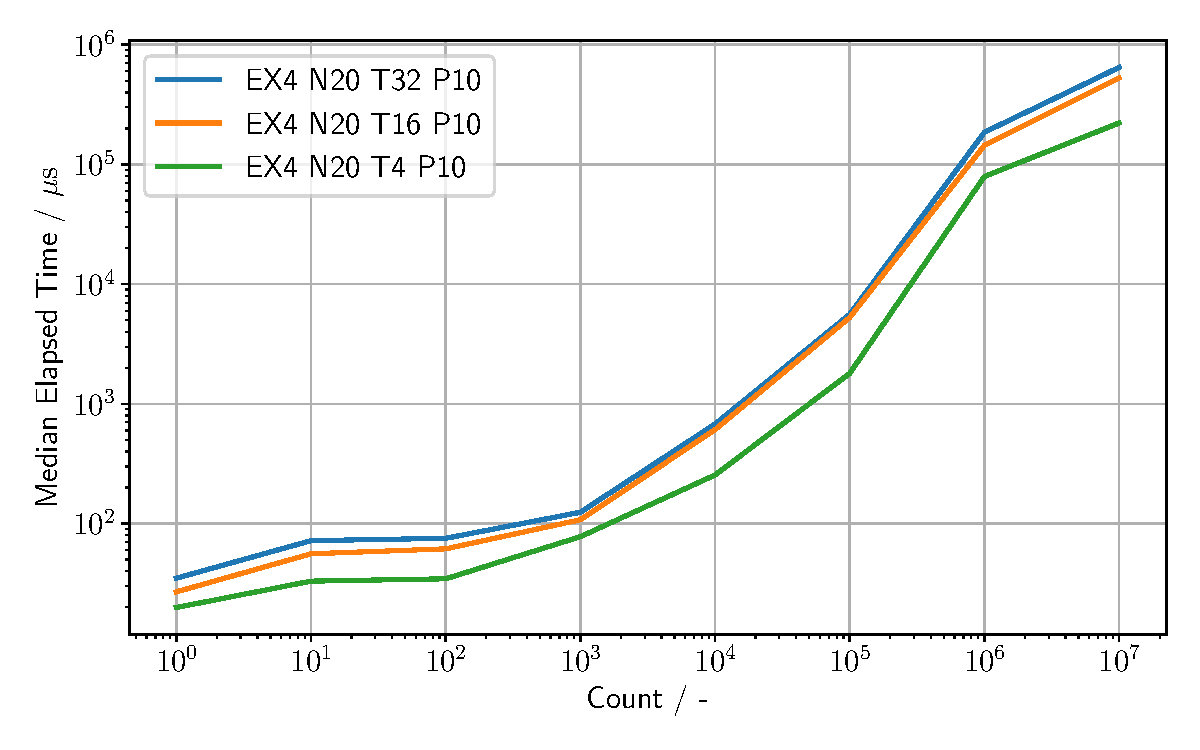
\includegraphics[width=1.0\linewidth]{figures/Ex4_3.pdf}
        \captionof{figure}{Caption for Ex2 plot 3}
        \label{Ex4_3_p}
    \end{minipage}%
    \begin{minipage}{.5\textwidth}
        \centering
        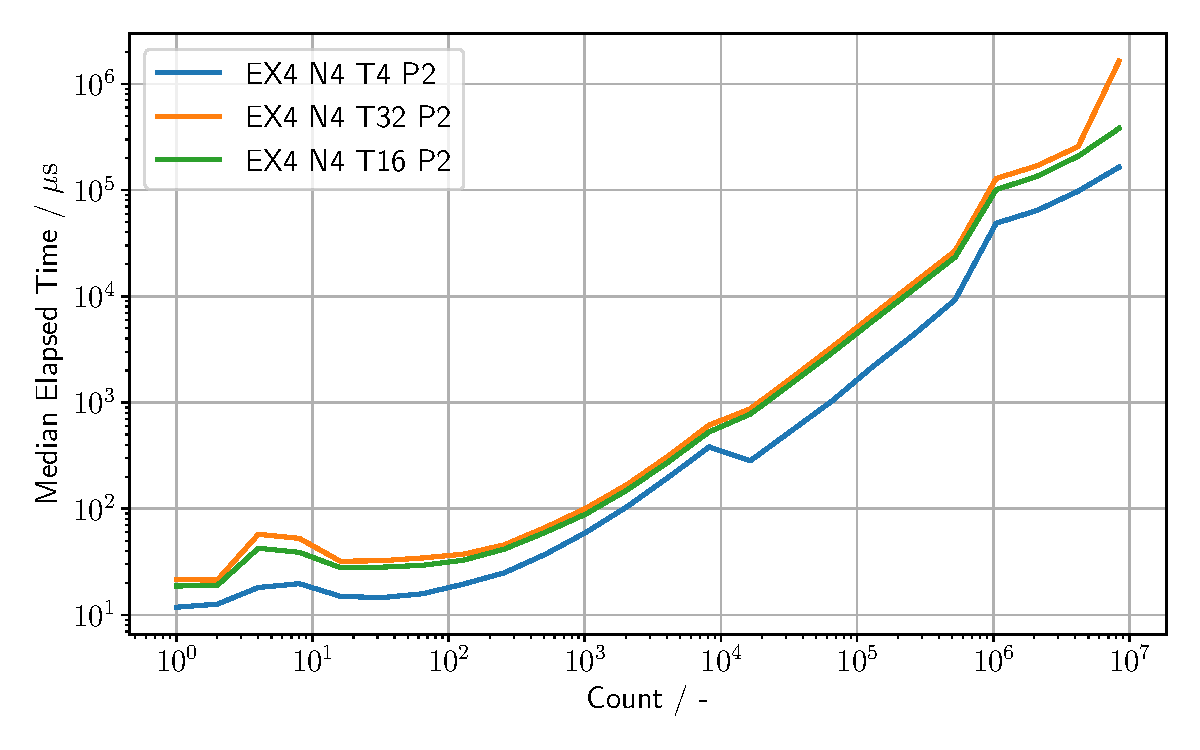
\includegraphics[width=1.0\linewidth]{figures/Ex4_4.pdf}
        \captionof{figure}{Caption for Ex4 plot 4}
        \label{Ex4_4_p}
    \end{minipage}
\end{figure}

\pagebreak

\section{Exercise 5 - Integrated, Improved Binary Tree Algorithm}

PROPER ZITAT VON TRAEFF 

We aim to devise an integrated, improved binary tree algorithm for \texttt{MPI\_Allreduce()}. Our 
implementation \texttt{MY\_Allreduce\_T()} is based on the algorithm for a doubly pipelined binary 
tree described in [Jesper Larsson Träff. A doubly-pipelined, dual-root reduction-to-all algorithm and 
implementation. arXiv:2109.12626, 2021.]. Note that we use only one tree, so there will never happen any 
communication between roots of different trees, as there is no. Per communication round, the reduction of 
one block can be performed. Hence, for complete reduction as much communication rounds are needed, 
as there are blocks. The idea is, that the root node starts with its broadcast-like send operations 
as soon as it received the data of the first block. The root node performs a local reduction against 
its own value and then the broadcasting starts while other blocks are still (or not yet) 
in their reduction phase. \\

\begin{figure}[h]
    \begin{center}
        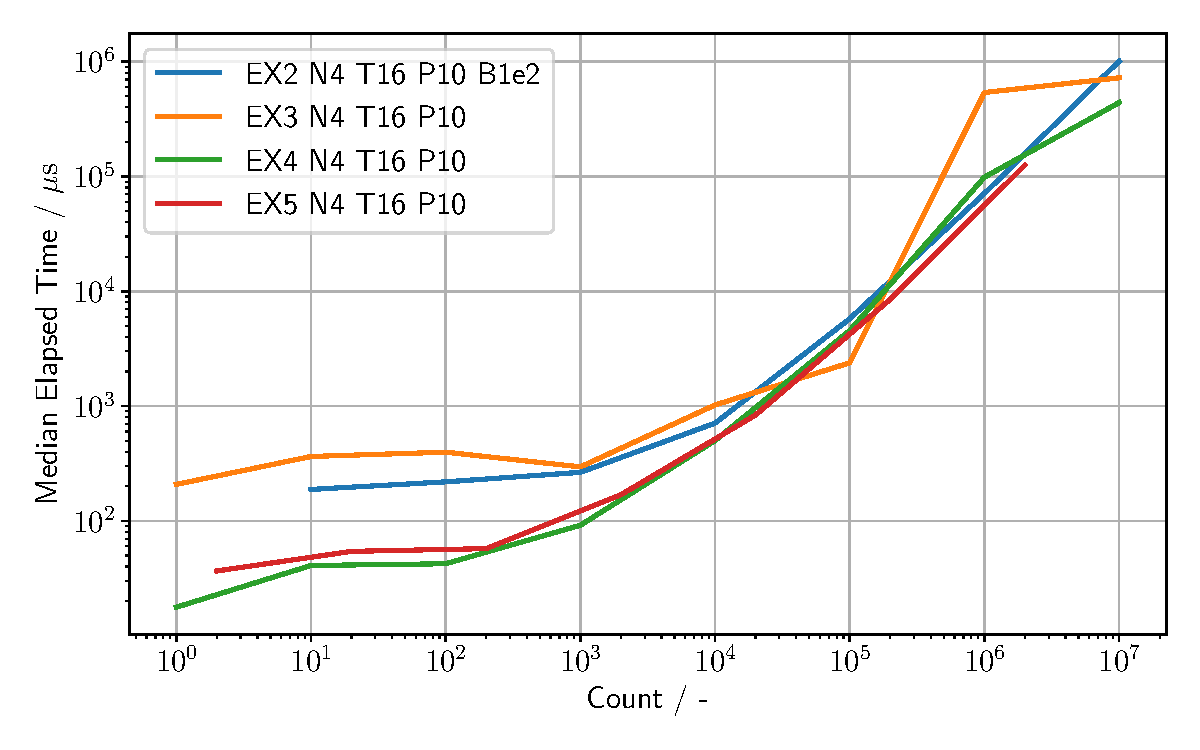
\includegraphics[width=1.0\linewidth]{figures/Ex5_3.pdf}
        \caption{Caption for Ex5 plot 3}
        \label{Ex5_3_p}
    \end{center}
\end{figure}

\begin{figure}[h]
\centering
    \begin{minipage}{.5\textwidth}
        \centering
        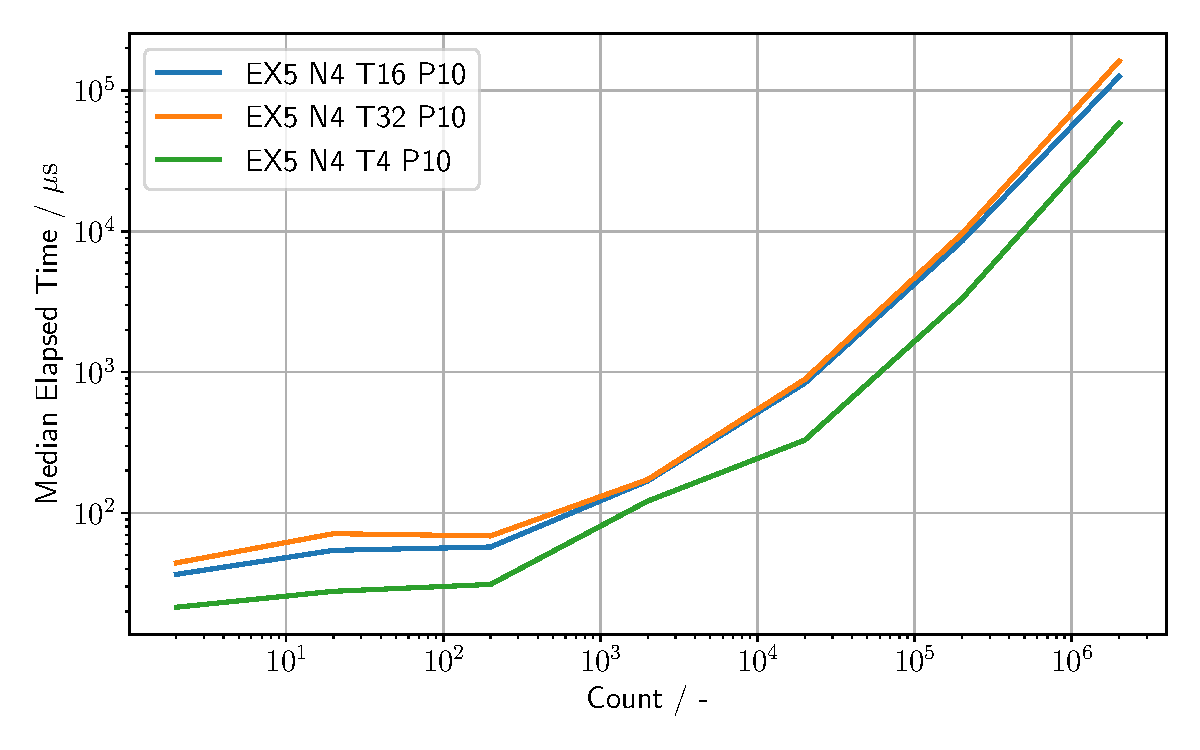
\includegraphics[width=1.0\linewidth]{figures/Ex5_1.pdf}
        \captionof{figure}{Caption for Ex5 plot 1}
        \label{Ex5_1_p}
    \end{minipage}%
    \begin{minipage}{.5\textwidth}
        \centering
        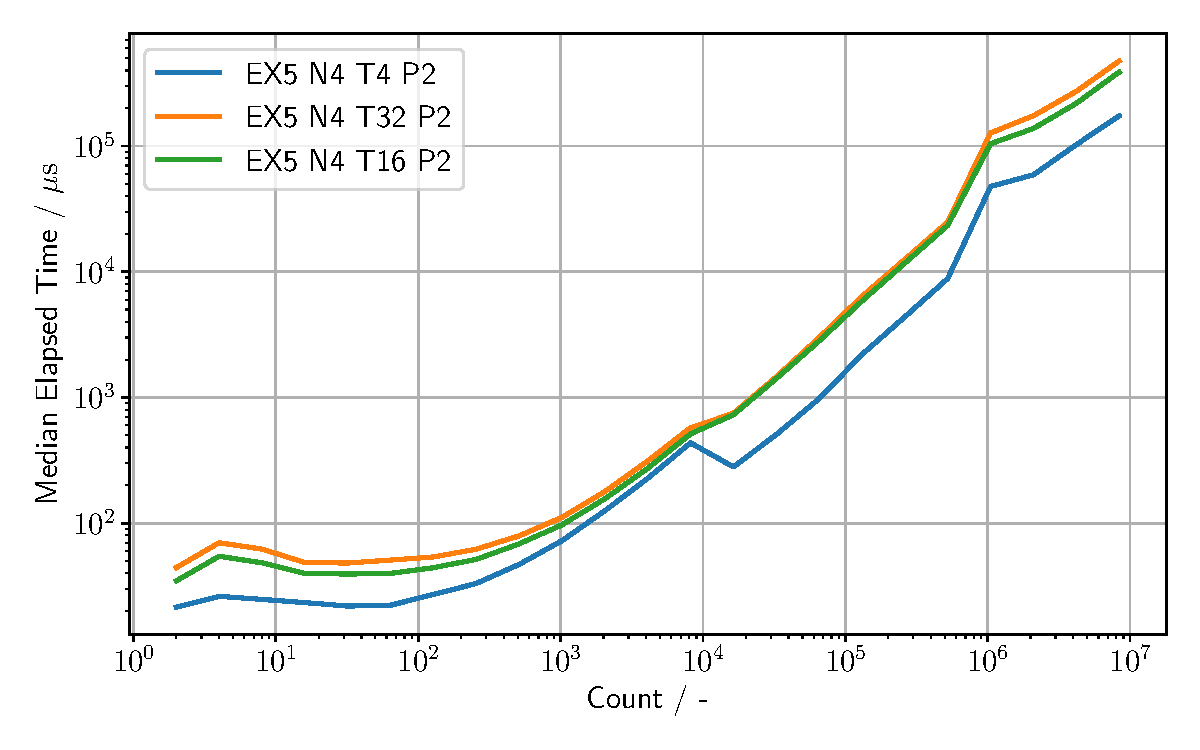
\includegraphics[width=1.0\linewidth]{figures/Ex5_2.pdf}
        \captionof{figure}{Caption for Ex5 plot 2}
        \label{Ex5_2_p}
    \end{minipage}
\end{figure}




\pagebreak

\section{Exercise 6 - Improvement with Sibling Leave Communication}
Not implemented.

\section{Exercise 7 - Implemenetation and Benchmarking of Improved Version}
Not implemented.

\pagebreak

%\section{Chapter 7}

%\pagebreak

%\section{Results and Conclusion}


\pagebreak
%%%%%%%%%%%%%%%%%%%%%%%%%%%%%%%%%%%%%%%%%%%%%%%%%%%%%%%%%%%
%%%%%%%%%%%%%%%%%%%%%%%%%%%%%%%%%%%%%%%%%%%%%%%%%%%%%%%%%%%
%%%%%%%%%%%%%%%%%%%%%%%%%%%%%%%%%%%%%%%%%%%%%%%%%%%%%%%%%%%
%%%%%%%%%%%%%%%%%%%%%%%%%%%%%%%%%%%%%%%%%%%%%%%%%%%%%%%%%%%


%% During the document writing process, this single .tex file is used to let dasdyou write down a little to do list, just comment it out when the paper is done!

%%%%%%%%%%%%%%%%%%%%%%%%%%%%%%%%%%%%%%%%%%%%%%%%%%%%%%%%%%%
%%%%%%%%%%%%%%%%%%%%%%%%%%%%%%%%%%%%%%%%%%%%%%%%%%%%%%%%%%%
%%%%%%%%%%%%%%%%%%%%%%%%%%%%%%%%%%%%%%%%%%%%%%%%%%%%%%%%%%%
%%%%%%%%%%%%%%%%%%%%%%%%%%%%%%%%%%%%%%%%%%%%%%%%%%%%%%%%%

%%% Bibliography printing at this point! 
\printbibliography

%%% This is a hardcoded string to enforce it in the table of contents, if you want your "references" string in the TOC to be named differently, such as bibliography or so on, just change the third input to this command below to your desired references naming that should appear in the TOC
%\addcontentsline{toc}{section}{References}


\pagebreak

%%%%%%%%%%%%%%%%%%%%%%%%%%%%%%%%%%%%%%%%%%%%%%%%%%%%%%%%%%%
%%%%%%%%%%%%%%%%%%%%%%%%%%%%%%%%%%%%%%%%%%%%%%%%%%%%%%%%%%%
%%%%%%%%%%%%%%%%%%%%%%%%%%%%%%%%%%%%%%%%%%%%%%%%%%%%%%%%%%%


%%% This is where the appendix .tex file is included, the settings to the appendix are changed in the settings.tex file
%\begin{appendix}
\addappheadtotoc
\section{CPP CUDA Code - Strided and Offset Memory Access - Task 1a}
\label{app_1a}

\begin{lstlisting}[language=C++, title=C++ Listing for EX1 a)]
#include <stdio.h>
#include "timer.hpp"
#include <algorithm>
#include <vector>

__global__ void addVec_kth(double *x, double *y, double *z, int N, int k) {
	unsigned int total_threads = blockDim.x * gridDim.x;
	unsigned int global_tid = blockIdx.x * blockDim.x + threadIdx.x;
	if (k==0) {
		k = 1;
	}
	for (unsigned int i = global_tid; i<N/k; i += total_threads) {
		z[i*k] = x[i*k] + y[i*k];
	}
}

// findMedian function for any vector lenghts, source geeksforgeeks.com
double findMedian(std::vector<double> a,
                  int n)
{
    if (n % 2 == 0) {
        std::nth_element(a.begin(),
                    a.begin() + n / 2,
                    a.end());
        std::nth_element(a.begin(),
                    a.begin() + (n - 1) / 2,
                    a.end());
        return (double)(a[(n - 1) / 2]
                        + a[n / 2])
               / 2.0;
    }
    else {
        std::nth_element(a.begin(),
                    a.begin() + n / 2,
                    a.end());
        return (double)a[n / 2];
    }
}

int main(void)
{
	// Task 1a//
	double *x, *y, *z, *gpu_x, *gpu_y, *gpu_z;
	double eff_BW;
	Timer timer;
	int N = pow(10.0, 8.0);
	std::vector<int> k_values(64, 0);
	for(int i = 0; i<64; i++){
		k_values[i] = i;
	}
	std::vector<double> exec_timings = {0, 0, 0, 0, 0, 0, 0, 0, 0, 0, 0};
	x = (double*)malloc(N*sizeof(double));
	y = (double*)malloc(N*sizeof(double));
	z = (double*)malloc(N*sizeof(double));
	for (int i = 0; i < N; i++) {
		x[i] = (double)(i);
		y[i] = (double)(N-i-1);
	}
	cudaMalloc(&gpu_x, N*sizeof(double)); 
	cudaMalloc(&gpu_y, N*sizeof(double));
	cudaMalloc(&gpu_z, N*sizeof(double));
	cudaMemcpy(gpu_x, x, N*sizeof(double), cudaMemcpyHostToDevice);
	cudaMemcpy(gpu_y, y, N*sizeof(double), cudaMemcpyHostToDevice);
	cudaMemcpy(z, gpu_z, N*sizeof(double), cudaMemcpyDeviceToHost);

	for (int i = 0; i < 64; i++) {
		for (int m = 0; m < 11; m++) {
			timer.reset();
			addVec_kth<<<256, 256>>>(gpu_x, gpu_y, gpu_z, N, k_values[i]);
			cudaDeviceSynchronize();
			exec_timings[m] = timer.get();
		}
		if (k_values[i]==0) {
			eff_BW = 3 * N * sizeof(double) * pow(10,-9) / findMedian(exec_timings, 10);
		}
		else{
			eff_BW = 3 * floor((N/k_values[i])) * sizeof(double) * pow(10, -9) / findMedian(exec_timings, 10);
		}
		printf("%d,%g\n", k_values[i], eff_BW);
	}

	cudaFree(gpu_x);
	cudaFree(gpu_y);
	cudaFree(gpu_z);
	free(x);
	free(y);
	free(z);
\end{lstlisting}
\pagebreak

\section{CPP CUDA Code - Offset Memory Access - Task 1b}
The code for the Offset Memory Access partial exercise is the same as for the
Strided Memory Access partial exercise, except the \texttt{\_\_global\_\_} part where
the offset is defined and the calculation of the effective bandwidth, where one can now
 also omit the case distinction for k=0.

\null

\label{app_1b}
\begin{lstlisting}[language=C++, title=C++ Listing for EX1 b)]
__global__ void addVec_kth(double *x, double *y, double *z, int N, int k) {
	unsigned int total_threads = blockDim.x * gridDim.x;
	unsigned int global_tid = blockIdx.x * blockDim.x + threadIdx.x;
	if (k==0) {
		k = 1;
	}
	for (unsigned int i = global_tid; i<N-k; i += total_threads) {
		z[i+k] = x[i+k] + y[i+k];
	}
}

.
.
.

eff_BW = 3 * floor((N - k_values[i])) * sizeof(double) * pow(10, -9) / findMedian(exec_timings, 10);

.
.
.

\end{lstlisting}

\pagebreak

\section{CPP CUDA Code - Dense Matrix Transpose - Task 2b}
\label{app_2b}

\begin{lstlisting}[language=C++, title=C++ Listing for EX2 b and c]
#include <stdio.h>
#include <iostream>
#include "timer.hpp"
#include "cuda_errchk.hpp"   // for error checking of CUDA calls

__global__
void transpose(double *A, double *B, int N)
{
  int t_idx = blockIdx.x*blockDim.x + threadIdx.x;
  int row_idx = t_idx / N;
  int col_idx = t_idx % N;
  
  if (row_idx < N && col_idx < N) B[row_idx * N + col_idx] = A[col_idx * N + row_idx];
}


void print_A(double *A, int N)
{
  for (int i = 0; i < N; i++) {
    for (int j = 0; j < N; ++j) {
      std::cout << A[i * N + j] << ", ";
    }
    std::cout << std::endl;
  }
}

int main(void)
{
  int N = 10;

  double *A, *cuda_A, *B, *cuda_B;
  Timer timer;

  // Allocate host memory and initialize
  A = (double*)malloc(N*N*sizeof(double));
  B = (double*)malloc(N*N*sizeof(double));
  
  for (int i = 0; i < N*N; i++) {
    A[i] = i;
  }

  print_A(A, N);


  // Allocate device memory and copy host data over
  CUDA_ERRCHK(cudaMalloc(&cuda_A, N*N*sizeof(double))); 
  CUDA_ERRCHK(cudaMalloc(&cuda_B, N*N*sizeof(double))); 

  // copy data over
  CUDA_ERRCHK(cudaMemcpy(cuda_A, A, N*N*sizeof(double), cudaMemcpyHostToDevice));

  // wait for previous operations to finish, then start timings
  CUDA_ERRCHK(cudaDeviceSynchronize());
  timer.reset();

  // Perform the transpose operation
  transpose<<<(N*N+255)/256, 256>>>(cuda_A, cuda_B, N);

  // wait for kernel to finish, then print elapsed time
  CUDA_ERRCHK(cudaDeviceSynchronize());
  double elapsed = timer.get();
  std::cout << std::endl << "Time for transpose: " << elapsed << std::endl;
  std::cout << "Effective bandwidth: " << (2*N*N*sizeof(double)) / elapsed * 1e-9 << " GB/sec" << std::endl;
  std::cout << std::endl;

  // copy data back (implicit synchronization point)
  CUDA_ERRCHK(cudaMemcpy(B, cuda_B, N*N*sizeof(double), cudaMemcpyDeviceToHost));

  print_A(B, N);

  cudaFree(cuda_A);
  cudaFree(cuda_B);
  free(A);
  free(B);

  CUDA_ERRCHK(cudaDeviceReset());  // for CUDA leak checker to work

  return EXIT_SUCCESS;
}
\end{lstlisting}


\end{appendix}



%%%%%%%%%%%%%%%%%%%%%%%%%%%%%%%%%%%%%%%%%%%%%%%%%%%%%%%%%%%
%%%%%%%%%%%%%%%%%%%%%%%%%%%%%%%%%%%%%%%%%%%%%%%%%%%%%%%%%%%
%%%%%%%%%%%%%%%%%%%%%%%%%%%%%%%%%%%%%%%%%%%%%%%%%%%%%%%%%%%


\end{document}

